\section{Proposta tecnológica}

Para o desenvolvimento do nosso sistema, precisamos de combinar um vasto conjunto de tecnologias que permitam 
simplificar o desenvolvimento de todas as funcionalidades propostas.

De forma a organizar o fluxo de trabalho do grupo, utilizamos o \href{https://trello.com/}{\textbf{Trello}}, 
que é um sistema para gestão de tarefas que segue o método \textit{kanban}, muito usado no desenvolvimento com \textit{Scrum}. 

\begin{figure}[H] 
  \centering
  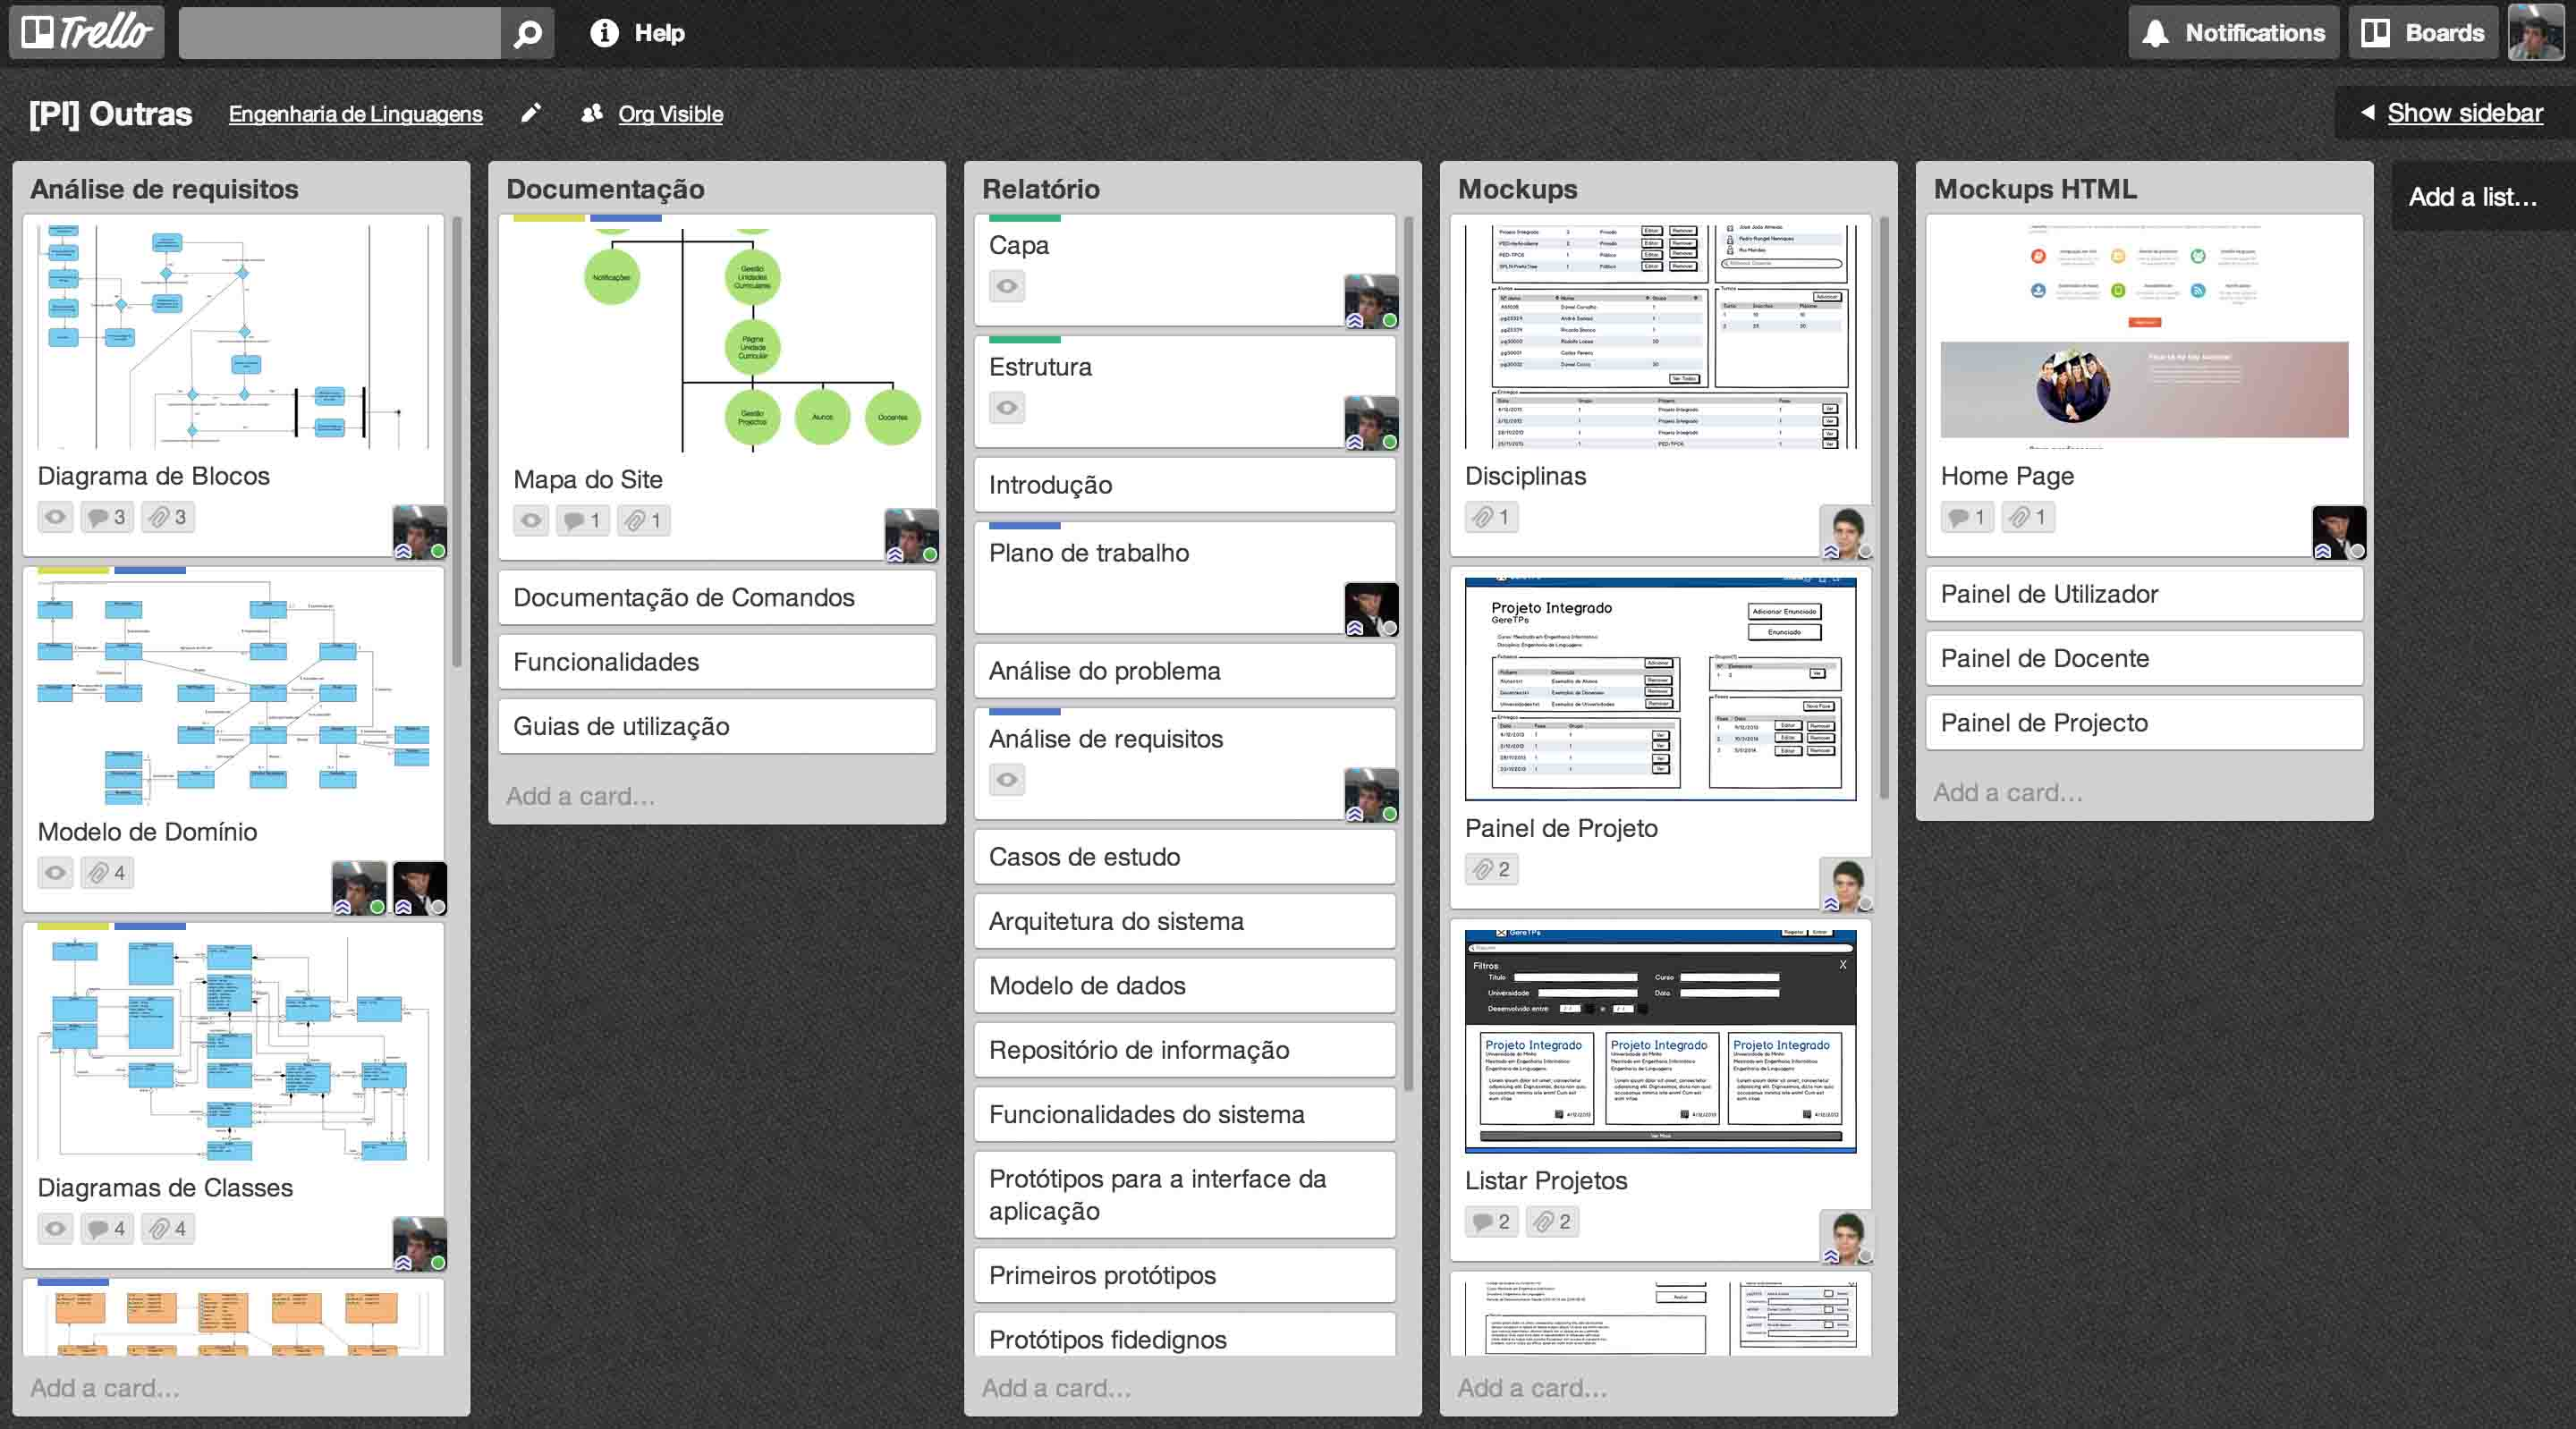
\includegraphics[width=1\textwidth]{images/tecnologias/trello}
  \caption{Trello}
  \label{fig:trello}
\end{figure}

Para o controlo de versões utilizaremos \textbf{Git}, que é um sistema de controlo de versões 
centralizado que apresenta as seguintes características:

\begin{itemize}
  \item Suporte consistente para desenvolvimentos não-lineares
  \item Desenvolvimento distribuído
  \item Compatibilidade com protocolos/sistemas existentes
  \item Manipulação eficiente de projetos extensos  
  \item Autenticação criptográfica do histórico 
  \item Modelo baseado em ferramentas 
  \item Estratégias de mescla (merge) conectáveis
  \item Empacotamento periódico explícito de objetos  
\end{itemize}

Para armazenar o código do nosso projeto vamos utilizar o \href{http://github.com}{\textbf{Github}}, 
que é um serviço de \textit{web hosting} o para projetos que usam o \textbf{Git} como sistema de controle de versões. 
Iremos utilizar um sistema de \textit{\textbf{Pull Requests}} e \textit{\textbf{Code Reviews}} 
para que assim todos os elementos possam ver e discutir o código produzido.

Procuraremos respeitar um dos fluxos de trabalho baseados em Git mais conhecidos, 
o \href{https://www.atlassian.com/git/workflows#!workflow-feature-branch}{\textbf{\textit{Feature Branch Workflow}}} 
que pode ser representado pela figura ~\ref{fig:git-workflow}.

\begin{figure}[H] 
  \centering
  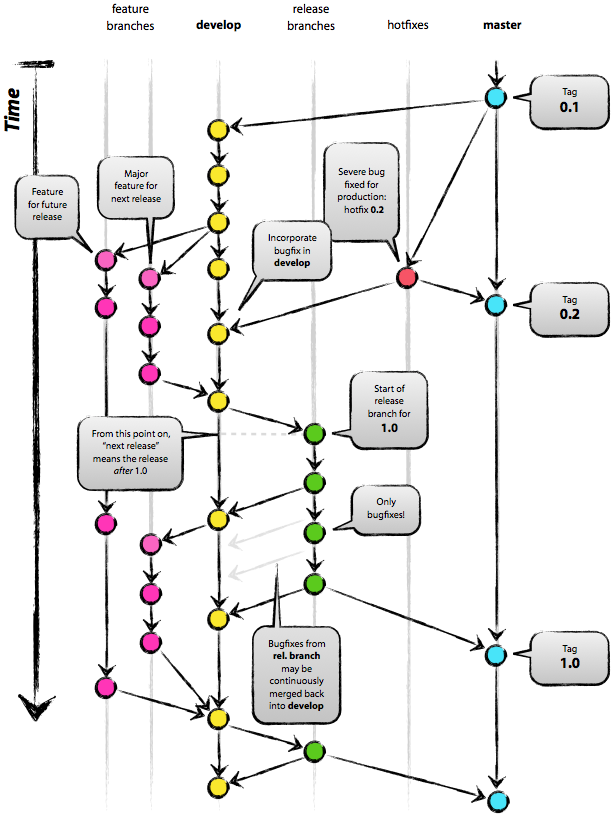
\includegraphics[width=0.5\textwidth]{images/tecnologias/git-workflow}
  \caption{Feature Branch Workflow}
  \label{fig:git-workflow}
\end{figure}

Rlativamente ao desenvolvimento, utilizaremos \href{http://rubyonrails.org/}{\textbf{Ruby on Rails}}, 
que é uma \textit{framework open-source} escrita em \textbf{Ruby}, otimizada para a produtividade sustentável. 
A \textit{framework} tem uma forte comunidade que defende conceitos como \textbf{DRY} \textit{(Don't Repeat Yourself)} 
e \textbf{\textit{Convention over configuration}}.

\textbf{Ruby on Rails} é uma \textit{meta-framework}, composta pelos seguintes \textbf{frameworks}:

\begin{description}[labelindent=1cm]
  \item[Active Record] Responsável pela interoperabilidade entre a aplicação e a base de dados, e pela abstração dos dados.
  \item[Action Pack] Compreende o \textbf{Action View} (gera o que o utilizador vê, como HTML, XML e JavaScript) 
  e o \textbf{Action Controller} (controle do fluxo de negócio).
  \item[Action Mailer] Responsável pelo serviço de entrega e receção de e-mails.
  \item[Active Support] Coleção de várias classes e bibliotecas, que foram considerados úteis para aplicações em Ruby on Rails.
\end{description}

Para além das \textit{frameworks} indicadas iremos recorrer a \textbf{Gems} para simplificar alguns processos, tais como:

\begin{description}[labelindent=1cm]
  \item[Devise] Autenticação de utilizadores.
  \item[Paperclip] Upload e validação de imagens e arquivos.
  \item[Capistrano] Automatização de processos de implantação \textit{(deployment)}.
  \item[Nokogiri] Parser de HTML e XML com XPath e seletores CSS.
  \item[XML-Simple] API simples para trabalhar com documentos XML.
\end{description} 

Pretendemos melhorar a nossa produtividade, e melhorar a legibilidade do código produzido utilizando os seguintes pré-processadores:

\begin{description}[labelindent=1cm]
  \item[\href{http://slim-lang.com/}{Slim}] para HTML.
  \item[\href{http://sass-lang.com/}{SASS}] para CSS.
  \item[\href{http://coffeescript.org/}{CoffeeScript}] para JavaScript.
\end{description} 

Utilizaremos também a \textit{framework} de \textit{front-end} \href{http://getbootstrap.com/}{\textbf{Twitter Bootstrap}} 
para ajudar a construirmos um serviço multi-plataforma e para reutilizarmos alguns componentes. 
E a biblioteca de Javascript \href{http://jquery.com/}{\textbf{JQuery}} para simplificar os \textit{scripts client side} que interagem com o HTML.\\

Para manipulação de documentos \textbf{XML}, utilizaremos as tecnologias lecionadas, tais como: \textbf{DTD}, \textbf{XSLT} e \textbf{XSD}.\\

Relativamente a tecnologias de Base de Dados, utilizaremos bases de dados SQL, mais especificamente \href{http://www.sqlite.org/}{\textbf{SQLite}} 
para ambientes de teste e desenvolvimento, e \href{http://www.postgresql.org/}{\textbf{PostgreSQL}} para ambientes de produção.



